\section{Uniqueness: the classification of covariant brackets}
\label{sec:classification}

\subsection{The three families}

Is the super-loop an accident of the octonions, or the only way to let spinor charges close into
Lorentz generators? We answer the question for every bracket that is covariant under the Lorentz group
$SL(2,\mathbb C)$ and the isospin group $SU(2)_{\rm v}$, with the spinor charges a Weyl spinor that is an
isodoublet, in three families:
\begin{itemize}
\item $\mathcal F^{\rm A}_{\rm LL}$ on $\mathfrak l_{\rm LL}\oplus\mathfrak s_{\rm LL}$ (real dimension 14);
\item $\mathcal F^{\rm B}_{\rm LL}$ on $\mathfrak l_{\rm LL}\oplus\mathfrak p_{\rm LL}\oplus\mathfrak s_{\rm LL}$
(18), with the translations $\mathfrak p_{\rm LL}$, the Hermitian bi-quaternions $\mathbf r=\mathbf
r^\dagger$, on which $\mathfrak l_{\rm LL}$ acts by $[\mathbf u,\mathbf r]=\mathbf u\mathbf r+\mathbf
r\mathbf u^\dagger$ (the Lorentz action on four-vectors);
\item $\mathcal F^{\rm C}_{\rm LL}$ on $\mathfrak l_{\rm LL}\oplus\mathfrak{su}(2)\oplus\mathfrak s_{\rm
LL}$ (17), with isospin generators $\mathbf t\in{\rm Im}\,\mathbb H$ as elements.
\end{itemize}
The bracket of $\mathfrak l_{\rm LL}$ with itself is the Lorentz bracket, and the other brackets are
\begin{align}
[\mathbf u,\mathbf b\mathbf e_4]&=c^{\rm tw}_{\rm LL}(W_{\rm LL}(\mathbf u)\mathbf b)\,\mathbf e_4,\nonumber\\
[\mathbf r,\mathbf r']&=c^{\rm PP}_{\rm LL}(\mathbf r\bar{\mathbf r}'-\mathbf r'\bar{\mathbf r}),\nonumber\\
[\mathbf r,\mathbf b\mathbf e_4]&=c^{\rm Ps}_{\rm LL}(\mathbf b^*\bar{\mathbf r})\,\mathbf e_4,\nonumber\\
[\mathbf t,\mathbf t']&=c^{\rm TT}_{\rm LL}(\mathbf t\mathbf t'-\mathbf t'\mathbf t),\label{eq:families}\\
[\mathbf t,\mathbf b\mathbf e_4]&=c^{\rm Ts}_{\rm LL}(\mathbf t\mathbf b)\,\mathbf e_4,\nonumber\\
[\mathbf b\mathbf e_4,\mathbf b'\mathbf e_4]&=c^{\rm sl}_{\rm LL}(\bar{\mathbf b}\mathbf b'-\bar{\mathbf b}'\mathbf b)\nonumber\\
&\quad+c^{\rm sP}_{\rm LL}\,i(\bar{\mathbf b}\mathbf b'^*-\bar{\mathbf b}'\mathbf b^*)\nonumber\\
&\quad+\mathrm{Re}\big[c^{\rm sT}_{\rm LL}(\mathbf b\bar{\mathbf b}'-\mathbf b'\bar{\mathbf b})\big],\nonumber
\end{align}
where a term is present only if its target sector is ($\mathfrak p_{\rm LL}$ in $\mathcal F^{\rm B}_{\rm
LL}$, $\mathfrak{su}(2)$ in $\mathcal F^{\rm C}_{\rm LL}$), the real part in the last term is taken
coefficient by coefficient so that the result lies in ${\rm Im}\,\mathbb H$, $c^{\rm sP}_{\rm LL}$ and
$c^{\rm TT}_{\rm LL}$ are real, and the other coefficients are complex. The bi-octonions are
$\mathcal F^{\rm A}_{\rm LL}$ with $c^{\rm tw}_{\rm LL}=-2$, $c^{\rm sl}_{\rm LL}=1$
(Eqs.~(\ref{eq:twist}) and~(\ref{eq:ss}); check M-1).

\emph{These brackets are the most general covariant ones.} Complexify: the Lorentz algebra becomes two
commuting copies of $\mathfrak{sl}(2)$, and a complex representation is labelled by its two spins. The
spinor charges are $(\tfrac12,0)$ times an isodoublet, their complex conjugates $(0,\tfrac12)$, the
Lorentz part $(1,0)$ with its conjugate $(0,1)$, the translations $(\tfrac12,\tfrac12)$ and the
isospin generators $(0,0)$ times an isotriplet. A covariant real bilinear bracket is a sum of covariant
complex-bilinear maps between these representations and their conjugates, and the number of such
maps is the number of times the target occurs in the tensor product of the sources: the target
$(\tfrac12,0)$ occurs once in $(1,0)\otimes(\tfrac12,0)$ and never in $(0,1)\otimes(\tfrac12,0)$ [the
twist $c^{\rm tw}_{\rm LL}$]; $(1,0)$ times the
isosinglet occurs once in the antisymmetric square of $(\tfrac12,0)$ times the isodoublet, and never in
$(\tfrac12,0)\otimes(0,\tfrac12)$ [$c^{\rm sl}_{\rm LL}$]; the antisymmetric square of
$(\tfrac12,\tfrac12)$ is $(1,0)\oplus(0,1)$ [$c^{\rm PP}_{\rm LL}$]; $(\tfrac12,0)$ occurs once in
$(\tfrac12,\tfrac12)\otimes(0,\tfrac12)$ and never in $(\tfrac12,\tfrac12)\otimes(\tfrac12,0)$, so the
bracket of a translation with a spinor charge is antilinear in the spinor [$c^{\rm Ps}_{\rm LL}$];
$(\tfrac12,\tfrac12)$ times the isosinglet occurs once in $(\tfrac12,0)\otimes(0,\tfrac12)$ times
isodoublet $\otimes$ isodoublet, and only one real combination is antisymmetric [$c^{\rm sP}_{\rm LL}$];
the isotriplet occurs once in the antisymmetric square of the spinor charges (spin 0, antisymmetric,
times isospin 1, symmetric) [$c^{\rm sT}_{\rm LL}$]; and the isodoublet occurs once in isotriplet
$\otimes$ isodoublet [$c^{\rm Ts}_{\rm LL}$]. All other brackets between different sectors vanish by
covariance. Each complex coefficient counts two real ones, as the reality of the bracket requires.

\subsection{Method}

The Jacobi identity and the linearized Malcev identity~(\ref{eq:malcev}) are multilinear, so they hold
for all elements if they hold for all basis elements. Evaluated on integer elements, each component of
an identity is a polynomial in the real and imaginary parts of the coefficients (degree 2 for Jacobi,
3 for Malcev). The script \texttt{malcev\_groebner.py} evaluates the identities of each family on
random integer tuples until the linear span of the resulting polynomials stops growing, and computes
the reduced Gr\"obner basis~\cite{CoxLittleOShea2015} of the ideal they generate,
$\mathcal I^{\rm Jac}_{\rm LL}$ for Jacobi and $\mathcal I^{\rm Mal}_{\rm LL}$ for Malcev
(Table~\ref{tab:groebner}). Every polynomial found is a true consequence of the identity, so a
polynomial that lies in the ideal vanishes on every solution: the statements below are necessary
conditions, proved by ideal membership. To restrict to solutions on which a polynomial does not
vanish (for example $c^{\rm sl}_{\rm LL}\neq0$), the ideal is enlarged by that polynomial times an
auxiliary variable $w^{\rm sat}_{\rm LL}$, minus 1 (saturation). Conversely, the Rust command
\texttt{malcev} checks every solution found here on \emph{all} basis triples and 4-tuples, in exact
integer arithmetic, so the solutions are proved to satisfy the identities (checks M-1 to M-9).

\begin{table}[t]
\caption{The constraint ideals: number of independent polynomials, of random integer tuples used, and
of elements of the reduced Gr\"obner basis (grevlex order), for each family and identity.}
\label{tab:groebner}
\begin{ruledtabular}
\begin{tabular}{lcccc}
family & identity & polynomials & tuples & basis\\
\hline
{{ROWS:groebner_table}}
\end{tabular}
\end{ruledtabular}
\end{table}

\subsection{Theorem M}

\noindent\emph{Theorem M.} (a) In $\mathcal F^{\rm A}_{\rm LL}$, the Jacobi identity forces $c^{\rm
sl}_{\rm LL}=0$ and $c^{\rm tw}_{\rm LL}\in\{0,1\}$ (G-1, G-2; Theorem L). (b) The Malcev identity
forces $c^{\rm tw}_{\rm LL}(c^{\rm tw}_{\rm LL}-1)(c^{\rm tw}_{\rm LL}+2)=0$, a cubic whose only roots
are $0$, $1$ and $-2$ (G-3); all three give Malcev algebras, the first two Lie algebras (M-2): the
value $-2$ is Carlsson's non-Lie Malcev module of $\mathfrak{sl}(2)$~\cite{Carlsson1976,Elduque1990}. If
$c^{\rm sl}_{\rm LL}\neq0$, then $c^{\rm tw}_{\rm LL}=-2$ (G-4), and the rescaling $\mathbf
b\mapsto\lambda^{\rm sc}_{\rm LL}\mathbf b$ by a complex number, which maps $c^{\rm sl}_{\rm LL}$ to
$(\lambda^{\rm sc}_{\rm LL})^2c^{\rm sl}_{\rm LL}$, makes $c^{\rm sl}_{\rm LL}=1$: the algebra is
$\mathfrak m_{\rm LL}$, the commutator algebra of the bi-octonions (M-1). Every other member fails
(M-3). (c) In $\mathcal F^{\rm B}_{\rm LL}$, even the Malcev identity forces $c^{\rm sl}_{\rm LL}=0$:
with translations present, spinor charges never close into Lorentz generators (G-7). The only non-Lie
Malcev member is $c^{\rm tw}_{\rm LL}=-2$ with all other coefficients zero (G-8, G-9, M-4, M-7): spinor
charges that commute with each other and with the translations, with the twisted Lorentz action. The
Lie members are (i) the Poincar\'e algebra with commuting spinor charges, (ii) the Poincar\'e algebra
with $[\mathfrak s_{\rm LL},\mathfrak s_{\rm LL}]\subset\mathfrak p_{\rm LL}$ ($c^{\rm sP}_{\rm LL}\neq0$),
and (iii) for $c^{\rm PP}_{\rm LL}=\lvert c^{\rm Ps}_{\rm LL}\rvert^2>0$ the de Sitter algebra
$\mathfrak{so}(4,1)$ (signature of its Killing form: 4 positive, 6 negative; M-6) acting on its real
spinor representation, with $[\mathfrak p_{\rm LL},\mathfrak s_{\rm LL}]\neq0$ and $[\mathfrak s_{\rm
LL},\mathfrak s_{\rm LL}]=0$ (G-5, G-6, M-5). (d) In $\mathcal F^{\rm C}_{\rm LL}$, the Jacobi identity
forces $c^{\rm sl}_{\rm LL}=0$ (G-10); and if $c^{\rm sl}_{\rm LL}\neq0$, the Malcev identity forces
$c^{\rm Ts}_{\rm LL}=c^{\rm sT}_{\rm LL}=0$ and $c^{\rm tw}_{\rm LL}=-2$ (G-11, G-12, M-8, M-9): isospin
cannot act on the spinor charges as an element of the algebra; it acts on the super-loop only from
outside, as the automorphisms~(\ref{eq:aut}).

The reduced Gr\"obner bases of $\mathcal F^{\rm A}_{\rm LL}$ illustrate the proof (variables: the real
and imaginary parts \texttt{ctw\_re}, \texttt{ctw\_im}, \texttt{csl\_re}, \texttt{csl\_im} of $c^{\rm
tw}_{\rm LL}$ and $c^{\rm sl}_{\rm LL}$). For the Jacobi identity the basis contains \texttt{csl\_re}
and \texttt{csl\_im} themselves---so $c^{\rm sl}_{\rm LL}=0$ on every solution---together with the real
and imaginary parts of $c^{\rm tw}_{\rm LL}(c^{\rm tw}_{\rm LL}-1)$. Case (ii) of (c) is a bosonic
analogue of supersymmetry: spinor charges whose brackets are translations. It is a Lie algebra, so the
theorem of Coleman and Mandula applies to it if it is to be a symmetry of a scattering matrix, and
Haag, {\L}opusza\'nski and Sohnius showed that the anticommutator, not the commutator, is the
consistent choice there. Case (iii) lives in de Sitter space, where the hypotheses H-dyn on a scattering
matrix are not available. Neither is a counterexample in the sense of this paper; they are listed to
make the classification complete.

\begin{figure}[t]
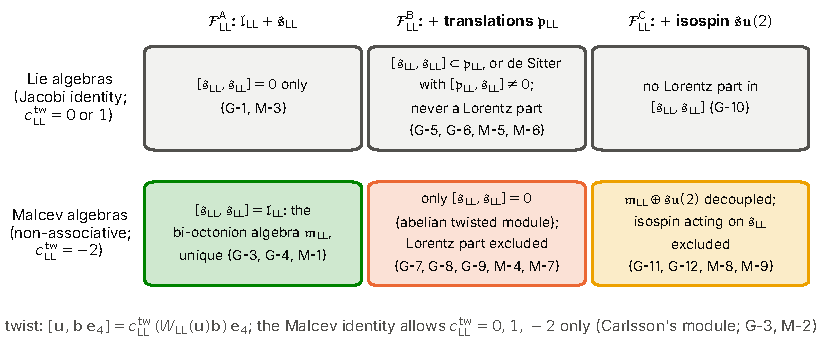
\includegraphics[width=\columnwidth]{../figures/fig_sl_classification.pdf}
\caption{Theorem M: what the bracket of two spinor charges can contain, for Lie algebras (top) and for
non-Lie Malcev algebras (bottom), in the three families. Green: the super-loop $\mathfrak m_{\rm LL}$,
unique; orange: the abelian twisted module of the Poincar\'e algebra; yellow: isospin decouples. The
labels are those of the checks.}
\label{fig:classification}
\end{figure}
